\documentclass[12pt]{article}
\usepackage[a4paper, total={5.5in, 8in}]{geometry}
\usepackage[utf8]{inputenc}
\usepackage{amsmath}
\usepackage{amsfonts}
\usepackage{amssymb}
\usepackage{graphicx}
\usepackage{mathtools}
\usepackage{hyperref}

\usepackage{listings}
\usepackage{color}
\definecolor{dkgreen}{rgb}{0,0.6,0}
\definecolor{gray}{rgb}{0.5,0.5,0.5}
\definecolor{mauve}{rgb}{0.58,0,0.82}

\lstset{frame=tb,
  language=Python,
  aboveskip=3mm,
  belowskip=3mm,
  showstringspaces=false,
  columns=flexible,
  basicstyle={\small\ttfamily},
  numbers=none,
  numberstyle=\tiny\color{gray},
  keywordstyle=\color{blue},
  commentstyle=\color{dkgreen},
  stringstyle=\color{mauve},
  breaklines=true,
  breakatwhitespace=true,
  tabsize=3
}



\newcommand{\qed}{\hfill $\blacksquare$}
\newcommand{\reals}{\mathbb{R}}
\newcommand{\complexes}{\mathbb{C}}



\author{Jacob Bruner}
\title{Logarithmic Analysis of Planetary Orbits}

\begin{document}
\maketitle
\tableofcontents
\pagebreak

\iffalse
############
heres an example of a code block
\begin{lstlisting}
        def intervalValues(z, n):
            return output # return the sequence of values
\end{lstlisting}

heres an example of an image
\begin{figure}[h]
\begin{center}
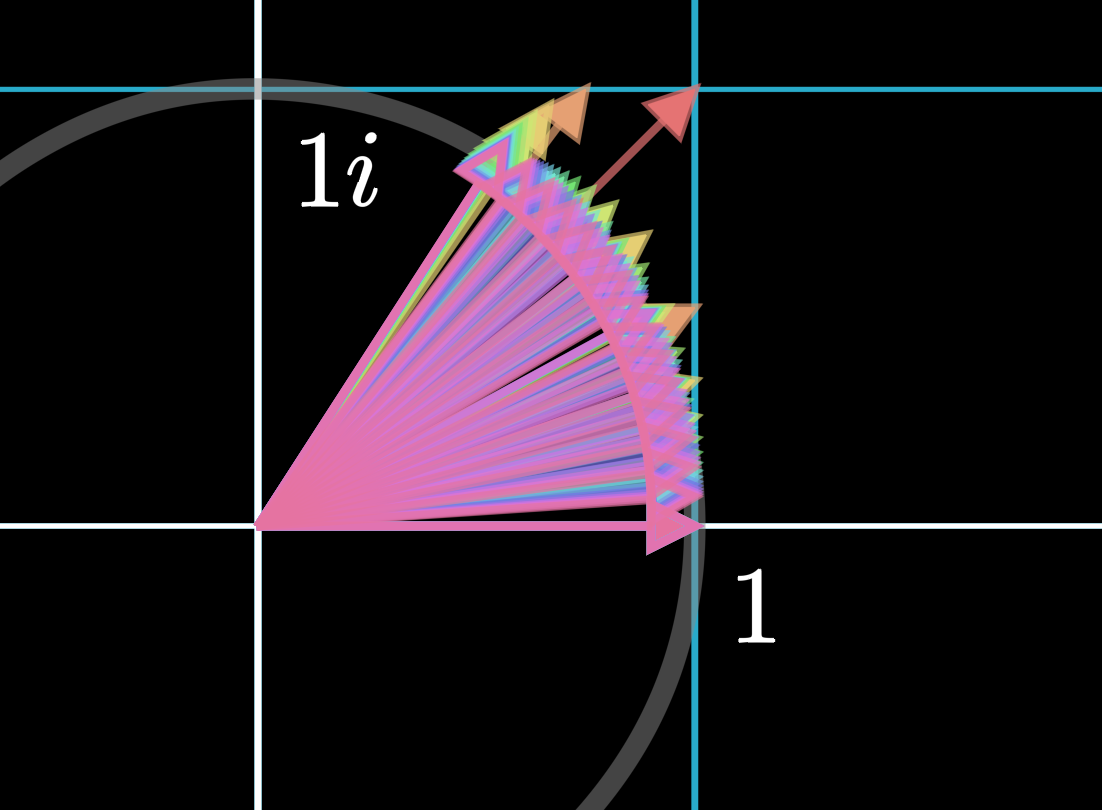
\includegraphics[scale=.37]{onefifteen} 
\caption{Sequences Generated by n = 1-15 on Argand Diagram}
\end{center}
\end{figure}
############
\fi

\section{Data Table}
\begin{table}[!ht]
    \centering
    \begin{tabular}{|l|l|l|}
    \hline
        Planet & radius (m) & Period (sec) \\ \hline \hline
        Mercury & 5.791E+10 & 7.601E+06 \\ \hline
        Venus & 1.082E+11 & 1.941E+07 \\ \hline
        Earth & 1.496E+11 & 3.156E+07 \\ \hline
        Mars & 2.279E+11 & 5.935E+07 \\ \hline
        Jupiter & 7.783E+11 & 3.744E+08 \\ \hline
        Saturn & 1.427E+12 & 9.293E+08 \\ \hline
        Uranus & 2.871E+12 & 2.651E+09 \\ \hline
        Neptune & 4.498E+12 & 5.200E+09 \\ \hline
    \end{tabular}
    \caption{Radius and Period of Planets in our Solar System \protect\footnotemark }
\end{table}
\footnotetext{ Planetary Systems Data, \href{https://www.princeton.edu/~willman/planetary_systems/Sol/}{https://www.princeton.edu/~willman/planetary\_systems/Sol/} }

Now to perform logarithmic analysis, we take the base ten logarithm of both Radius and Period like so:
\begin{align*}
LR_{Murcury} &= \log_{10} ( R_{Mercury} ) \\
LR_{Murcury} &= \log_{10} ( 5.79 \times 10^{10}\ m) \\
LR_{Murcury} &= 10.793 \ \log (m)
\end{align*}

Calculating for the remaining data points:\\

\begin{table}[!ht]
    \centering
    \begin{tabular}{|l|l|l|}
    \hline
        Planet & log radius (log(m)) & log period (log(sec)) \\ \hline \hline
        Mercury & 10.763 & 6.881 \\ \hline
        Venus & 11.034 & 7.288 \\ \hline
        Earth & 11.175 & 7.499 \\ \hline
        Mars & 11.358 & 7.773 \\ \hline
        Jupiter & 11.891 & 8.573 \\ \hline
        Saturn & 12.154 & 8.968 \\ \hline
    \end{tabular}
     \caption{Base 10 Logarithm of Radius and Period of Planets in Solar System}
\end{table}
\vspace*{1cm}
\pagebreak

\section{Graphs}

\begin{figure}[h]
\begin{center}
\hspace*{-1cm} 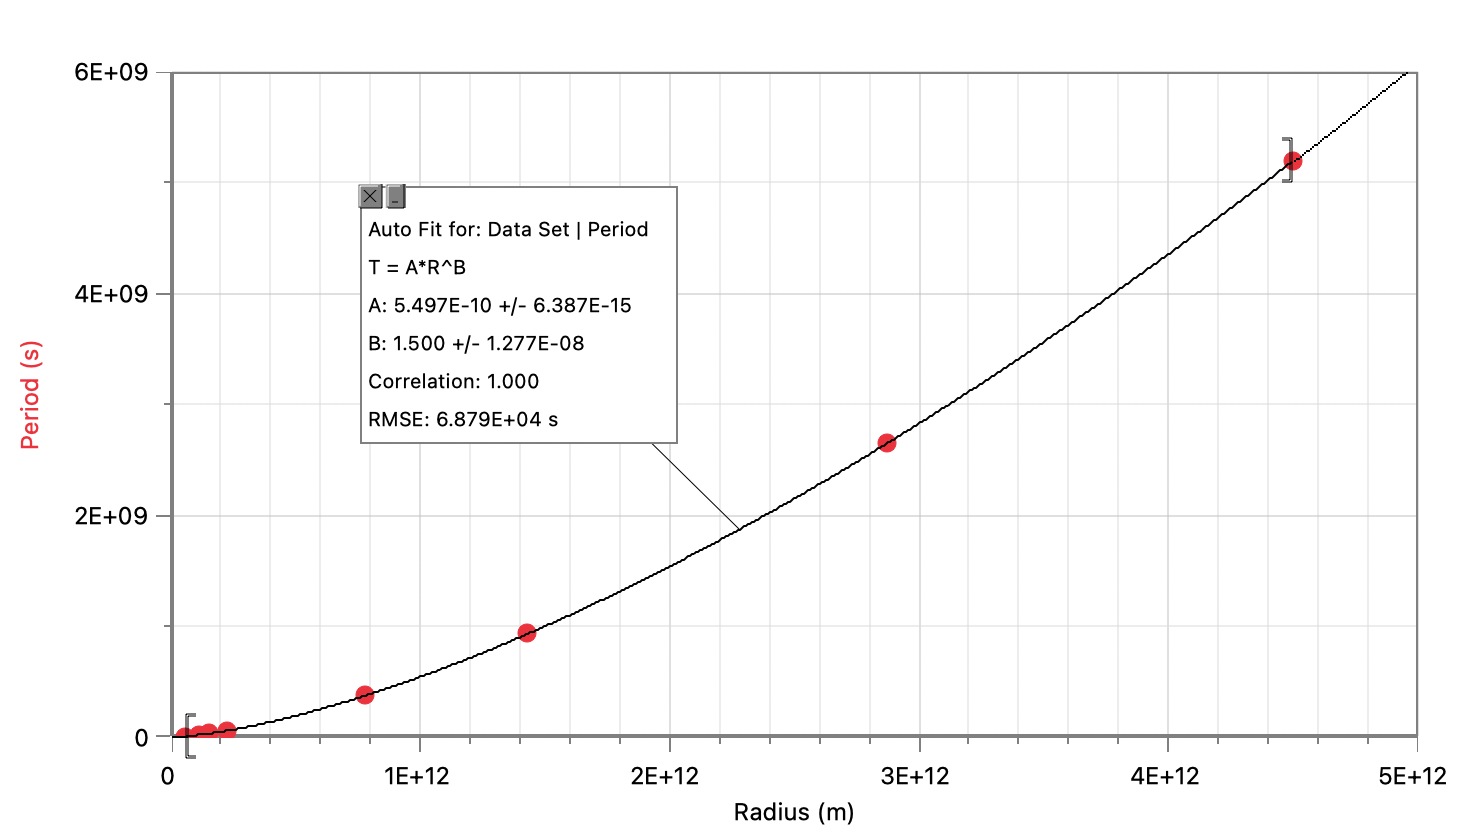
\includegraphics[scale=.60]{graph} 
\caption{The Effect of Planetary Period on Orbital Radius of Planets in our Solar System}
\end{center}
\end{figure}

In Figure 1, the data was plotted with Period on the Y-axis and Radius on the X-axis.  The data points for each planet is plotted in red. Running a Power Law regression in Logger Pro, we obtain, to three significant figures, the equation of best fit: $ T\  (sec) = (5.50\times 10^{-10})\  r^{1.50} $
\pagebreak
\begin{figure}[h]
\begin{center}
\hspace*{-1cm} 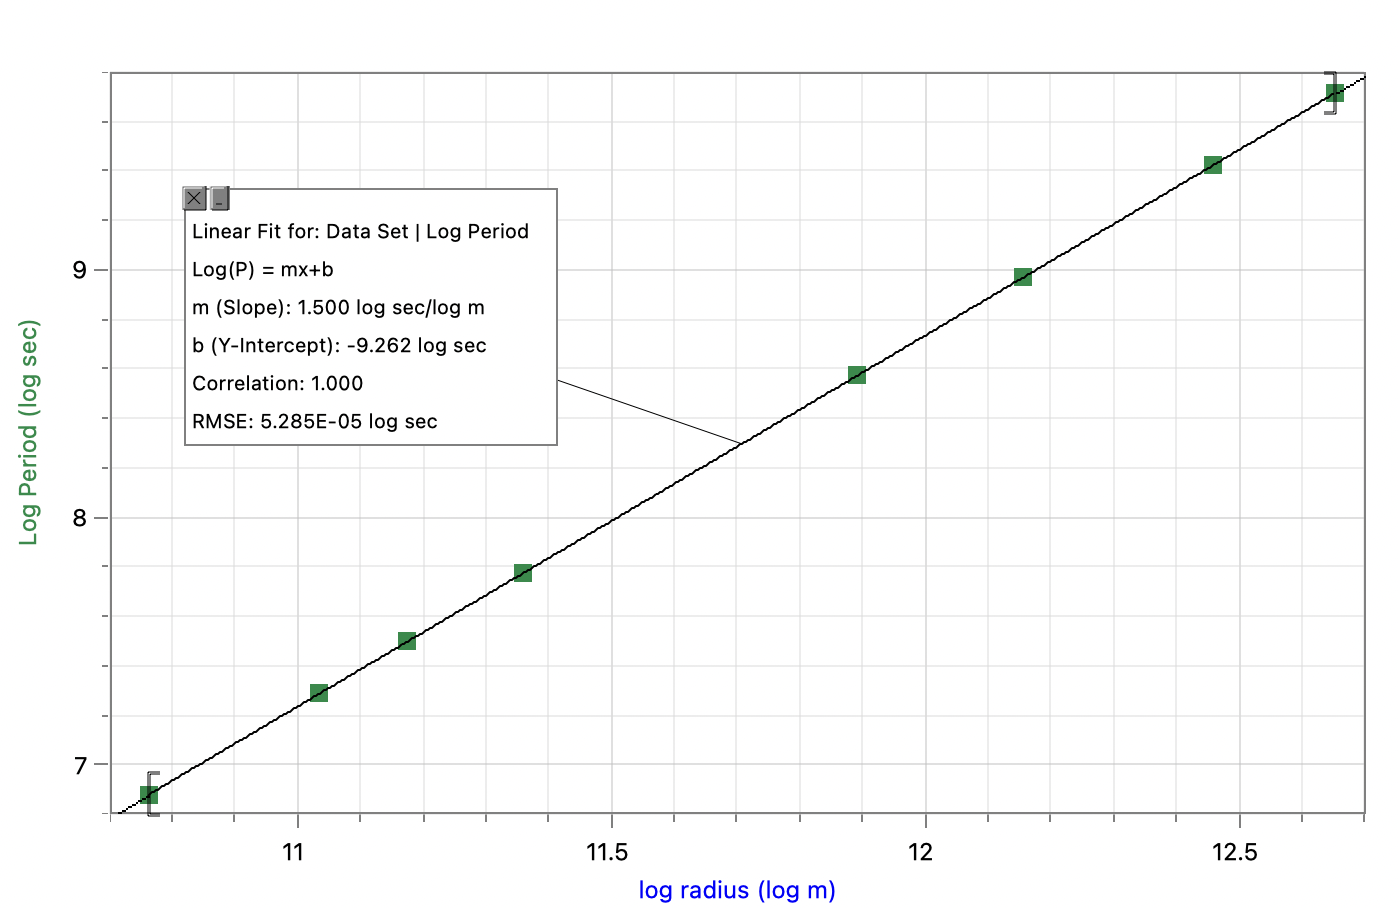
\includegraphics[scale=.60]{log graph} 
\caption{The Effect of Logarithmic Planetary Period on Logarithmic Orbital Radius of Planets}
\end{center}
\end{figure}

Using the data from table 2 to obtain a log–log graph, we can linearize the power law relationship and determine the appropriate power and coefficients from its slope and intercept like so:
\begin{align*}
T &= \alpha r^{\beta} \\
\log{T} &= \log{\alpha r^{\beta}} \\
\log{T} &= \log{ r^{\beta}}  +  \log{\alpha} \\
\underbrace{\log{T}}_{y} &= \underbrace{ \beta ( \log{ r}) + \log{\alpha} }_{mx + b}
\end{align*}

\begin{align*}
\beta &= 1.500 \\
\log_{10}{\alpha} &= -9.262 \\
\Rightarrow \alpha &= 5.497 \times 10^{-10} \\
\Rightarrow T\ (sec) &= (5.50 \times 10^{-10}) \ r^{1.50}
\end{align*}

\pagebreak
\section{Predicting Values}

To evaluate a predicted formula relating orbital period as a function of radius (assuming a circular orbit), first consider the force-balance between the gravitational force and the centripetal force acting on the planet.  Solving for velocity $v$ given the mass of the star $M$,  the mass of the planet $m$, the radius of orbit $r$ and the gravitational constant $G$:

\begin{align}
F_g &= F_c \nonumber \\ 
\frac{GMm}{r^2} &= \frac{mv^2}{r} \nonumber \\ 
\Rightarrow \ v^2 &= \frac{GM}{r} \nonumber \\
v &= \sqrt{\frac{GM}{r}} 
\end{align}

Now consider the formula for the period of revolution around a circumference $2 \pi r$ and the magnitude of the velocity $v$:
 
 \begin{align}
 T &= \frac{2 \pi r}{v} 
 \end{align}

From here, we can substitute (1) into (2) and simplify to yield the formula required. 

 \begin{align}
 T &= \frac{2 \pi r}{\sqrt{\frac{GM}{r}}} \nonumber \\
 T &= \frac{2 \pi r \sqrt{r}}{\sqrt{GM}} \nonumber \\
 T &= 2 \pi \sqrt{\frac{r^3}{GM}} \nonumber \\
 T &= \frac{2 \pi}{\sqrt{GM}} \times  r^{\frac{3}{2}}
\end{align}

Now to evaluate the accuracy of the experiment, the mass of the sun and the gravitational constant can be used to determine a predicted coefficient of $r^\frac{3}{2}$.  Hence using the known value of G, the gravitational constant,  and M, the mass of the sun, to four significant figures and substituting into (3):

 \begin{align*}
 T &= \frac{2 \pi}{\sqrt{ \big( 6.674 \times 10^{-11}\ N\ m^2\ kg^{-2} \big) \big( 	1.9885 \times 10^{30} \ kg \big) }} \times  r^{\frac{3}{2}} \\
 T &= (5.4540 \times 10^{-10}) \times  r^{\frac{3}{2}}
\end{align*}

This coefficient deviates only slightly from the experimental value determined by the log–log analysis $(5.497 \times 10^{-10})$. We can determine the percent error like so:

\begin{align*}
\% Error &= \frac{ | Theoretical-Experimental | }{Theoretical} \\
&= \frac{ | (5.454 \times 10^{-10}) - ( 5.497 \times 10^{-10} ) | }{5.454 \times 10^{-10}} \\
&= 0.789 \%
\end{align*}

Therefore, the value determined by the log–log analysis reflects a high degree of accuracy compared to the theoretical derivation. 

\section{Comparing Experimental and Theoretical}

In both the power rule regression and the slope of the linearized log–log graph,  the experimental value of the radius' exponent was accurate to a great extent.  Compared to the theoretical value of exactly $\frac{3}{2}$ or $1.5$, the power law regression determined the exponent was $1.500 \pm 1.277 \times 10^{-8}$, evidently demonstrating a supposed accuracy to the one hundred millionth decimal place.  Similarly, the slope of the log–log graph was calculated by the software to be 1.500. Hence, to the software's accuracy of four significant figures, the experimental exponent is equivalent to the theoretical exponent to a high degree of confidence.


\end{document}
